\documentclass[compress,11pt]{beamer}
%\includeonly{pendel}
\usetheme{Ilmenau}
%\usetheme{fau-4-3}
%\usecolortheme{beaver}
\beamertemplatenavigationsymbolsempty
\usepackage[ngerman]{babel}
\usepackage{marvosym}
\usepackage{multimedia}
\usepackage[utf8]{inputenc}
\usepackage{amsmath}
\usepackage{amsfonts}
\usepackage{amssymb}
\usepackage{graphicx}
\usepackage{esvect}
%\author{}
\title{EP Gruppe 8}
%\setbeamercovered{transparent}
%\setbeamertemplate{navigation symbols}{}
%\logo{}
%\institute{}
%\date{}
%\subject{}
\usepackage{verbatim}
\begin{document}

\begin{frame}

Schaltbild Filter 2. Ordnung, Erste Stufe:\\
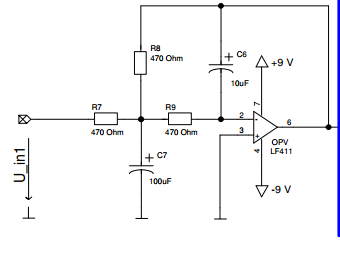
\includegraphics[width=.7\textwidth]{schalt/schalt_41}

\end{frame}

\begin{frame}
\begin{block}{Eigenschaften des Tschebyscheff-Filters}
\begin{itemize}
\item Im Vergleich zum passiven Filter 2. Ordnung: Einsatz vim Operationsverstärkern(Filter daher auch aktiv genannt)
\item Verlauf des Bode-Diagramms entspricht Tschebyscheff-Polynomen
\item daher im Bereich der Grenzfrequenz auch kein Monotoner Verlauf, sondern Welligkeit, bedingt dur verstärkenden Schwingkreis
\item Dämpfung immer um $40 \frac{dB}{Dekade}$
\item Cut-Off-Frequenz für den zweiten Filter: $f = 32 Hz$
\end{itemize}
\end{block}



\end{frame}

\begin{frame}
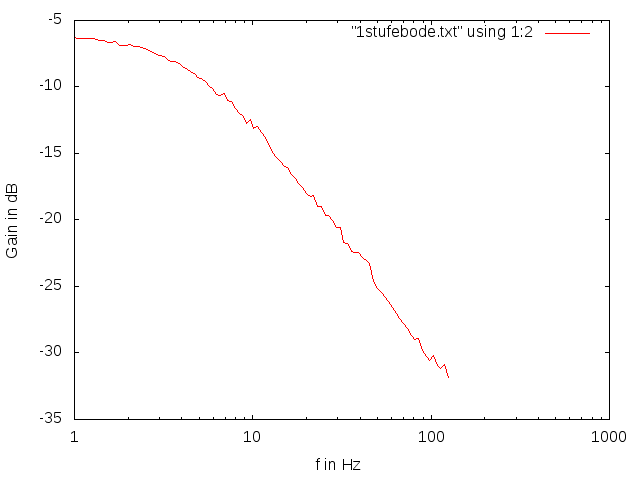
\includegraphics[width=.7\textwidth]{4aufgabe/1stufegain}\\
Gain-Bodediagramm der ersten Stufe
\end{frame}
\begin{frame}
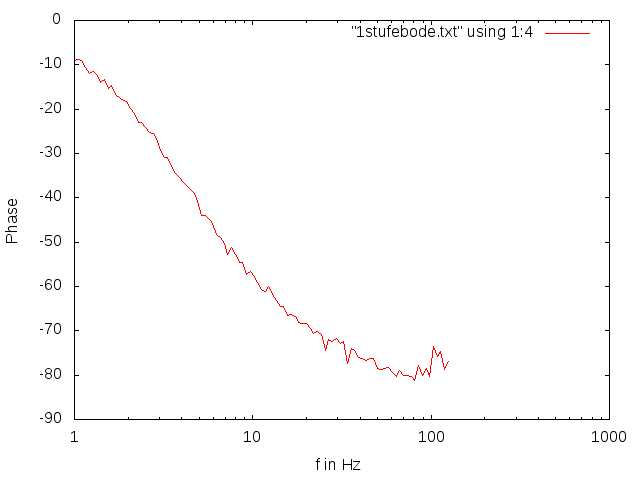
\includegraphics[width=.7\textwidth]{4aufgabe/1stufephase}\\
Phase-Bodediagramm der ersten Stufe
\end{frame}



\begin{frame}
Schaltbild Filter 2. Ordnung, Zweite Stufe:\\
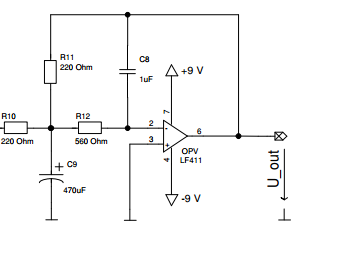
\includegraphics[width=.7\textwidth]{schalt/schalt_42}
\end{frame}




\begin{frame}
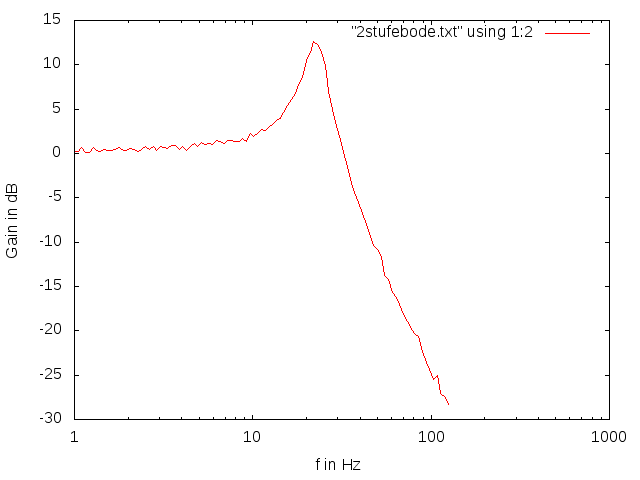
\includegraphics[width=.7\textwidth]{4aufgabe/2stufegain}\\
Gain-Bodediagramm der zweiten Stufe
\end{frame}
\begin{frame}
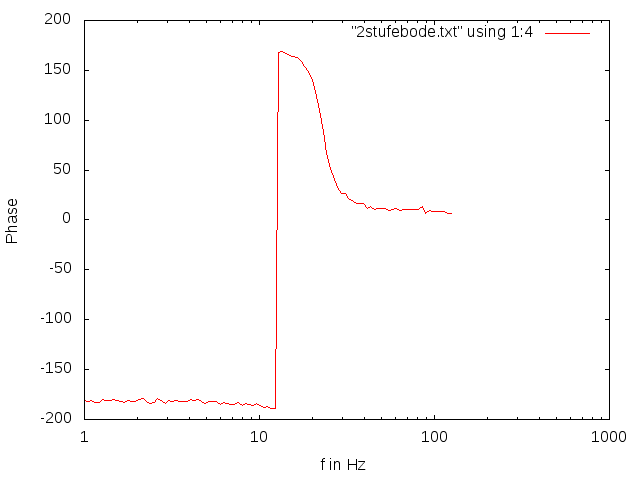
\includegraphics[width=.7\textwidth]{4aufgabe/2stufephase}\\
Phase-Bodediagramm der zweiten Stufe
\end{frame}
\begin{frame}
Ablesen der Grenzfrequenz und der Welligkeit bei Stufe 1 nicht möglich, da Gain zu tiefe Werte annimmt\\
Dämpfung: $V \approx 20 \frac{dB}{Dekade}$\\
Für Stufe 2 ergibt sich:\\
Welligkeit $W \approx 12.6 dB$ bei $f_W \approx	22 Hz$\\
Grenzfrequenz: $f \approx 35 Hz$
Dämpfung: $V > 30 \frac{dB}{Dekade}$



\end{frame}
\begin{frame}
\begin{block}{Theorie für Filter 4. Ordnung}
Dämpfung ergibt sich aus Überlagerungen der Einzeldämpfungen
$\Rightarrow$ $V = 80 \frac{dB}{Dekade}$\\
Für Cut-Off-Frequenz erhält man: $f = 23.3 Hz$
\end{block}
\end{frame}
\begin{frame}
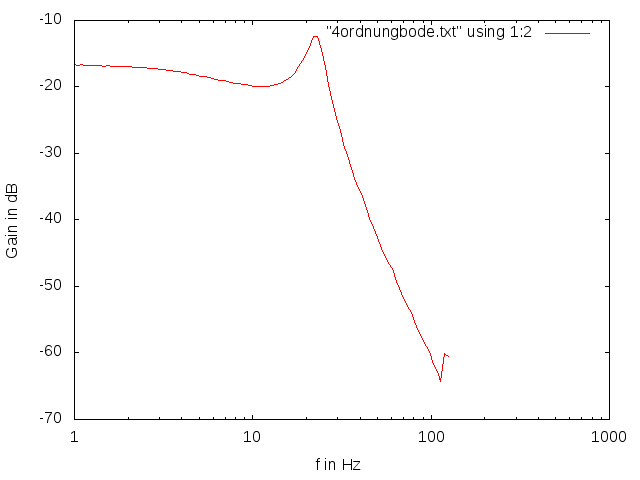
\includegraphics[width=.7\textwidth]{4aufgabe/4stufegain}\\
Gain-Bodediagramm des Gesamtfilters\\
Auffällig ist, dass das ganze Bode-Diagramm nach unten versetzt ist und zb. nie den Wert $-3 dB $ erreicht
\end{frame}
\begin{frame}
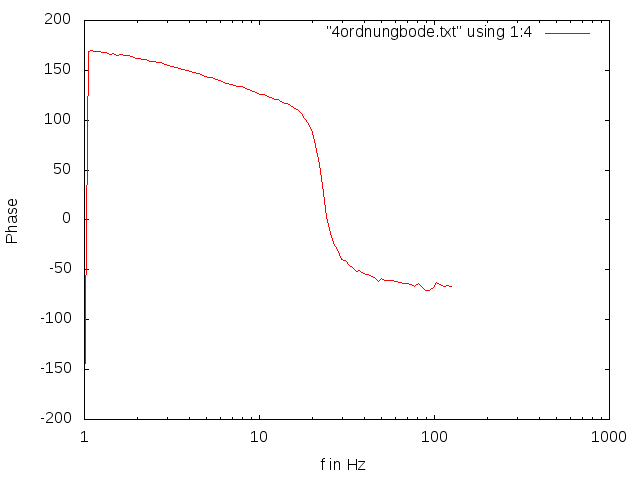
\includegraphics[width=.7\textwidth]{4aufgabe/4stufephase}\\
Phase-Bodediagramm des Gesamtfilters
\end{frame}
\begin{frame}
Dämpfung $V \approx 55 \frac{dB}{Dekade}$\\
Welligkeit: suche $A_{min} = -12.3 dB$ und berechne $A_{peak} - A_{min}$. Man erhält: $W \approx 4.4 dB$
bei $f_W \approx 23.06 Hz$
\end{frame}
\begin{frame}

\end{frame}
\end{document}